\chapter{Rezultaty}
\section{Dobór parametrów algorytmu}
%\begin{itemize}
%\item tabelki z wyselekcjonowanymi parametrami, takie jak w excelu
%%\item wykres dla Schaffer1 bestfitness_calych_scenariuszy_Schaffer1 
%%\item fitness_etapow_scenariuszymutDefault_Schaffer1
%%\item fitness_etapow_scenariuszymutGauss_Schaffer1
%\end{itemize}
Przed przystąpieniem do badań porównujących efektywność badanych algorytmów konieczne jest określenie najlepszych ich konfiguracji. Dobór wartości parametrów algorytmów oparto na procedurze opisanej w podrozdziale \ref{sec:badane_scenariusze_doboru_parametrow}. Zdecydowano się na osobną selekcję parametrów dla każdej z wykorzystanych funkcji testowych co w rezultacie pozwoliło na uzyskanie konfiguracji przedstawionych w tabelach \ref{table:selekcja_Schaffer_parametry}, \ref{table:selekcja_Paviani_parametry} i \ref{table:selekcja_Zeldasine_parametry}. Analizując tabele pierwszym spostrzeżeniem będącym potwierdzeniem intuicji jest fakt uzyskiwania lepszych rezultatów przez algorytmy oparte na większych populacjach. Dlatego w większości przypadków przyjęta konfiguracja składa się z maksymalnej rozpatrywanej liczby osobników. Zdominowanie parametru metody przeszukiwania lokalnego w algorytmach memetycznych przez metodę \emph{L-BFGS-B}, która jest domyślną wartością w implementacji pakietu \emph{GA} może być konsekwencja przyjętej miary porównawczej konfiguracji algorytmów. Już na poziomie dokumentacji pakietu pojawia się uwaga mówiąca, że \emph{L-BFGS-B} najczęściej uzyskuje najlepsze rezultaty, jednakże nie jest najszybszym z operatorów. Uwzględnienie czasu wykonania algorytmu jako współkryterium dla uzyskiwanego rozwiązania w procedurze selekcji parametrów algorytmów mogłoby w rezultacie przynieść potrzebę zmiany przyjmowaną metodę przeszukania lokalnego.

\begin{table}[ht]
\caption{Dobrane wartości parametrów algorytmów dla funkcji \emph{Schaffer nr 2}}
\label{table:selekcja_Schaffer_parametry}
\begin{center}
\begin{tabular}{|c|c|c|c|c|c|c|c|}
	\hline
	Algorytm & Mutacja & $p_{mut}$ & $p_{cross}$ & $r_{pop}$ & $p_{opt}$ & $p_{sel}$ & Operator\\
	\hline
	Memetyczny & \emph{mutDefault} & 0.5 & 0.9 & 100 & 0.8 & 1.0 & \emph{L-BFGS-B} \\
	Memetyczny & \emph{mutGauss}  & 0.7 & 0.9 & 100 & 1.0 & 0.6 & \emph{L-BFGS-B} \\
	Genetyczny & \emph{mutDefault} & 0.6 & 0.9 & 100 & - & - & - \\
	Genetyczny & \emph{mutGauss}  & 0.5 & 1.0 & 100 & - & - & - \\
	\hline
	\end{tabular}

\begin{tabular}{|c|c|c|c|c|}
	\hline
	Algorytm & $\phi_1$ & $\phi_2$ & $w$ & $r_{pop}$ \\
	\hline
	PSO & 1.6 & 2.5 & 1.0 & 100 \\
	\hline
\end{tabular}
\end{center}
\end{table}
  
\begin{table}[ht]
\caption{Dobrane wartości parametrów algorytmów dla funkcji \emph{Paviani}}
\label{table:selekcja_Paviani_parametry}
\begin{center}
\begin{tabular}{|c|c|c|c|c|c|c|c|}
	\hline
	Algorytm & Mutacja & $p_{mut}$ & $p_{cross}$ & $r_{pop}$ & $p_{opt}$ & $p_{sel}$ & Operator\\
	\hline
	Memetyczny & \emph{mutDefault} & 0.5 & 0.7 & 100 & 1.0 & 1.0 & \emph{L-BFGS-B} \\
	Memetyczny & \emph{mutGauss}  & 0.8 & 0.9 & 100 & 1.0 & 0.9 & \emph{L-BFGS-B} \\
	Genetyczny & \emph{mutDefault} & 0.8 & 0.7 & 100 & - & - & - \\
	Genetyczny & \emph{mutGauss}  & 1.0 & 1.0 & 100 & - & - & - \\
	\hline
	\end{tabular}

\begin{tabular}{|c|c|c|c|c|}
	\hline
	Algorytm & $\phi_1$ & $\phi_2$ & $w$ & $r_{pop}$ \\
	\hline
	PSO & 1.0 & 3.1 & 0.8 & 100 \\
	\hline
\end{tabular}
\end{center}
\end{table}

\begin{table}[ht]
\caption{Dobrane wartości parametrów algorytmów dla funkcji \emph{ZeldaSine10}}
\label{table:selekcja_Zeldasine_parametry}
\begin{center}
\begin{tabular}{|c|c|c|c|c|c|c|c|}
	\hline
	Algorytm & Mutacja & $p_{mut}$ & $p_{cross}$ & $r_{pop}$ & $p_{opt}$ & $p_{sel}$ & Operator\\
	\hline
	Memetyczny & \emph{mutDefault} & 0.7 & 1.0 & 100 & 0.6 & 0.6 & \emph{L-BFGS-B} \\
	Memetyczny & \emph{mutGauss}  & 0.9 & 1.0 & 50 & 1.0 & 0.6 & \emph{L-BFGS-B} \\
	Genetyczny & \emph{mutDefault} & 0.8 & 0.9 & 100 & - & - & - \\
	Genetyczny & \emph{mutGauss}  & 0.9 & 1 & 100 & - & - & - \\
	\hline
	\end{tabular}

\begin{tabular}{|c|c|c|c|c|}
	\hline
	Algorytm & $\phi_1$ & $\phi_2$ & $w$ & $r_{pop}$ \\
	\hline
	PSO & 1.6 & 2.5 & 1.0 & 100 \\
	\hline
\end{tabular}
\end{center}
\end{table}

\par
W tabelach \ref{table:selekcja_Schaffer_czasy}, \ref{table:selekcja_Paviani_czasy} i \ref{table:selekcja_Zeldasine_czasy} zaprezentowano uśrednione najlepsze rozwiązanie znajdowane przy wykorzystaniu wyselekcjonowanych konfiguracji algorytmów w ramach selekcji, tj. przy wykorzystaniu zaledwie 5 pierwszych pokoleń. W przypadku algorytmów memetycznych przedstawiono również który z omówionych w podrozdziale \ref{sec:badane_scenariusze_doboru_parametrow} scenariuszy ostatecznie uzyskał najlepsze rezultaty. W  tym miejscu można zauważyć zależność pomiędzy trudnością funkcji testowe i kompletnością zwycięskiego scenariusza. Dokładna analiza wykonania algorytmu memetycznego dla funkcji \emph{Zeldasine10} wykazała, że wykorzystany operator \emph{L-BFGS-B} bardzo szybko znajduje optymalne rozwiązanie. W takiej sytuacji, gdzie wiele scenariuszy pozwala na osiąganie optimum funkcji kluczowym parametrem wyboru scenariusza staje się czas jego wykonania. 

\begin{table}[ht]
\caption{Czasy i najlepsze rozwiązanie znalezione w trakcie selekcji parametrów algorytmów dla funkcji \emph{Schaffer nr 2}}
\label{table:selekcja_Schaffer_czasy}
\begin{center}
\begin{tabular}{|c|c|c|c|c|}
	\hline
	Algorytm & Mutacja & Najlepsze rozwiązanie & Czas selekcji [s] & Scenariusz \\
	\hline
	Memetyczny & \emph{mutDefault} & 0.03788 & 540.74 & $[1-2-3,\; 4-5-6]$\\
	Memetyczny & \emph{mutGauss} & 0.02769 & 584.67 & $[1-2-3,\; 4-5-6]$ \\
	Genetyczny & \emph{mutDefault} & 0.06609 & 171.79 & - \\
	Genetyczny & \emph{mutGauss} & 0.04549 & 186.90 & - \\
	PSO	& - & 0.09882 & 282.22 & -\\

	\hline
	\end{tabular}
\end{center}
\end{table}            

\begin{table}[ht]
\caption{Czasy i najlepsze rozwiązanie znalezione w trakcie selekcji parametrów algorytmów dla funkcji \emph{Paviani}}
\label{table:selekcja_Paviani_czasy}
\begin{center}
\begin{tabular}{|c|c|c|c|c|}
	\hline
	Algorytm & Mutacja & Najlepsze rozwiązanie & Czas selekcji [s] & Scenariusz \\
	\hline
	Memetyczny & \emph{mutDefault} & -45.77847 & 849.00 & $[4-5-6,\; 1-2-3]$\\
	Memetyczny & \emph{mutGauss} & -45.77847 & 841.99 & $[4-5-6,\; 1-2-3]$ \\
	Genetyczny & \emph{mutDefault} & -24.71857 & 212.64 & - \\
	Genetyczny & \emph{mutGauss} & -23.36381 & 218.80 & - \\
	PSO	& - & -37.78442 & 412.75 & -\\

	\hline
	\end{tabular}
\end{center}
\end{table}




\begin{table}[ht]
\caption{Czasy i najlepsze rozwiązanie znalezione w trakcie selekcji parametrów algorytmów dla funkcji \emph{ZeldaSine10}}
\label{table:selekcja_Zeldasine_czasy}
\begin{center}
\begin{tabular}{|c|c|c|c|c|}
	\hline
	Algorytm & Mutacja & Najlepsze rozwiązanie & Czas selekcji [s] & Scenariusz \\
	\hline
	Memetyczny & \emph{mutDefault} & -3.5 & 243.22 & $[4-5,\;3-6,\;1-2]$\\
	Memetyczny & \emph{mutGauss} & -3.5 & 190.31 & $[4-5,\;3-6,\;1-2]$ \\
	Genetyczny & \emph{mutDefault} & -1.69261 & 206.83 & - \\
	Genetyczny & \emph{mutGauss} & -1.81252 & 214.95 & - \\
	PSO	& - & -0.91760 & 36.15 & -\\

	\hline
	\end{tabular}
\end{center}
\end{table}

Jednym z celów realizowanej pracy było sprawdzenie skuteczności zaproponowanych w rozdziale \ref{ch:przyjety_model_doboru_parametrow_algorytmu} scenariuszy doboru kolejnych wartości parametrów algorytmów memetycznych w celu ograniczenia liczby sprawdzanych kombinacji bez znaczącej straty jakości przyjętej konfiguracji. Z powodu ograniczeń technicznych nie zdecydowano się na porównawcze wykonanie pełnego przeglądu wszystkich możliwych kombinacji, więc scenariusze porównane zostaną jedynie między sobą pod kątem uzyskanych rezultatów i czasu wykonania. W tym miejscu na wykresach \ref{fig:parameter_selection_fitness_overall}, \ref{fig:parameter_selection_fitness_in_phases}, \ref{fig:parameter_selection_time_overall} i \ref{fig:parameter_selection_time_in_phases} przedstawione zostało jedynie porównanie dla funkcji \emph{Schaffer nr 2}. Analogiczne wykresy dla pozostałych przyjętych funkcji testowych zamieszczono w dodatku \ref{ch:dodatekC-wykresy}.
\par
Jak przedstawiono na wykresie \ref{fig:parameter_selection_fitness_overall} konfiguracja uzyskana poprzez zastosowanie scenariusza $[1-2-3,\,4-5-6]$ pozwala na uzyskanie najlepszych rezulatów, jednakże scenariusz $[3-6,\,1-2,\,4-5]$ jest tylko nieznacznie gorszy w tym aspekcie. Dodatkowo porównując wspomniane dwa scenariusze na podstawie wykresu \ref{fig:parameter_selection_time_overall} można stwierdzić, że uzyskanie nieznacznie lepszego rozwiązania wymagało aż trzykrotnie dłuższych obliczeń. Zestawiając ze sobą te dwa wyróżniające się pod kątem jakości uzyskanej konfiguracji scenariusze stwierdzić, że oba z nich są równie użyteczne, ale w odniesieniu do różnych potrzeb wykorzystania. Jeśli priorytetem będzie maksymalna możliwa jakość parametrów algorytmów to lepszym będzie scenariusz $[1-2-3,\,4-5-6]$, natomiast jeśli ważniejszy będzie czas selekcji parametrów to $[3-6,\,1-2,\,4-5]$. Zdecydowanie się na szybszy scenariusz może pozwolić na zwiększenie zbiorów sprawdzanych wartości parametrów, a przez to zwiększenie jakości uzyskanej konfiguracji algorytmu. Należy jednak po raz kolejny zaznaczyć, że skuteczność scenariuszy bezpośrednio zależy od trudności optymalizowanej funkcji.
\par
Analizując wykres \ref{fig:parameter_selection_fitness_in_phases} przedstawiający rezultaty uzyskane w kolejnych etapach selekcji można zauważyć niespodziewane wyniki dla scenariusza $[4-5,\,3-6,\,1-2]$ z operatorem \emph{mutDefault} oraz $[1-2-3,\,4-5-6]$ z \emph{mutGauss} wskazujące na to, że przeprowadzony kolejny etap selekcji pogorszył otrzymywane rozwiązanie. Może to wskazywać na sytuację, w której przy danej kombinacji pozostałych parametrów tymczasowo przyjęte domyślne wartości parametrów pozwalają na uzyskanie lepszych rezultatów niż którakolwiek z testowanych kombinacji danego etapu selekcji. Gdyby taka sytuacja była obserwowana w większej liczbie scenariuszy lub rozwiązanie w kolejnych etapach pogarszałoby się w znaczący sposób należałoby zmienić zakres testowanych wartości parametrów w stronę domyślnych zaimplementowanych w pakiecie \emph{GA}.
\par
W sytuacji, gdy jakość konfiguracji uzyskana najlepszym pod tym kątem scenariuszem nie jest wystarczająca można posłużyć się danymi czasu wykonania kolejnych etapów selekcji przedstawionymi na wykresie \ref{fig:parameter_selection_time_in_phases}. Przedstawia on czas wykonania kolejnych etapów selekcji. Na tej podstawie można zdecydować, któremu z parametrów można rozszerzyć zbiór sprawdzanych wartości bez diametralnego wydłużenia czasu wykonania całego scenariusza. Z drugiej strony, jeśli celem jest skrócenie czasu wykonania scenariusza na podstawie wykresu można określić, zbiory których parametrów należy ograniczyć.
\begin{figure}[h] 
\centering
  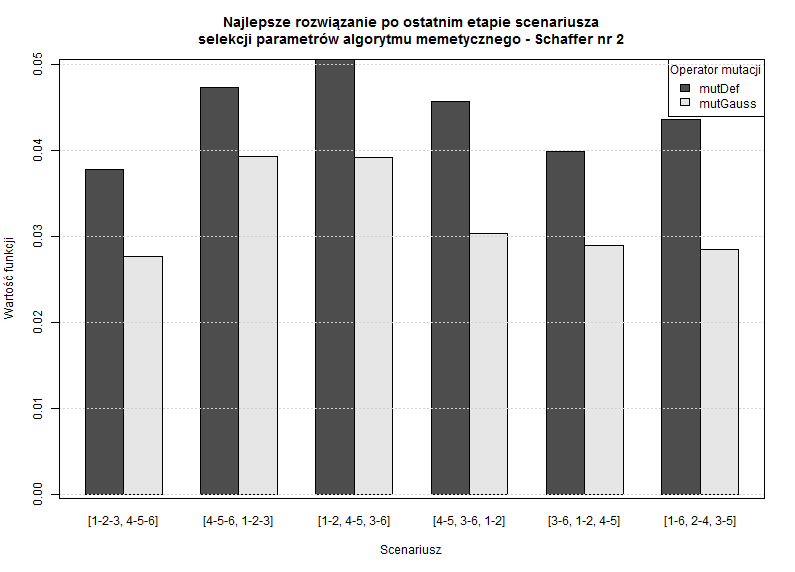
\includegraphics[width=\linewidth]{{img//roz04//parameterSelection//bestfitness_calych_scenariuszy_Schaffer1.png}}
\caption{Porównanie najlepszego rozwiązania dla różnych scenariuszy dla funkcji \emph{Schaffer nr 2}}
\label{fig:parameter_selection_fitness_overall}
\end{figure}


\begin{figure}[ht] 
\centering
\begin{subfigure}{\textwidth}
  \centering
  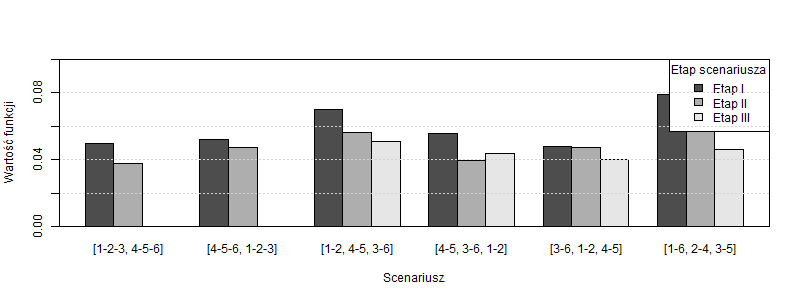
\includegraphics[width=\linewidth]{{img//roz04//parameterSelection//fitness_etapow_scenariuszymutDefault_Schaffer1.png}}
  \caption{\emph{mutDefault}}
  %\label{fig:sub1}
\end{subfigure}
\begin{subfigure}{\textwidth}
  \centering
  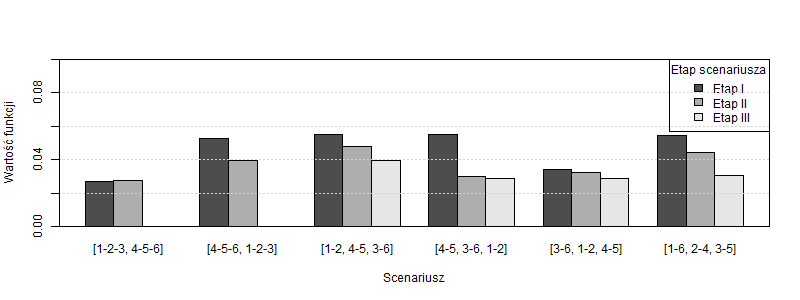
\includegraphics[width=\linewidth]{img//roz04//parameterSelection//fitness_etapow_scenariuszymutGauss_Schaffer1.png}
  \caption{\emph{mutGauss}}
  %\label{fig:sub2}
\end{subfigure}
\caption{Najlepsze znajdywane rozwiązanie kolejno w etapach selekcji dla funkcji \emph{Schaffer nr 2}}
\label{fig:parameter_selection_fitness_in_phases}
\end{figure}

\begin{figure}[h] 
\centering
  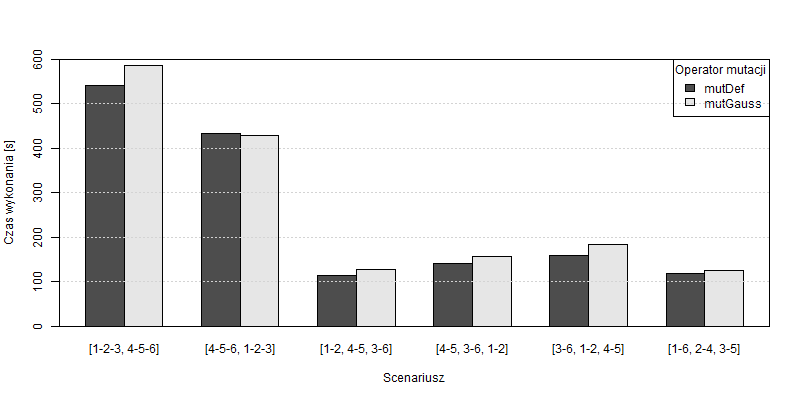
\includegraphics[width=\linewidth]{{img//roz04//parameterSelection//czas_calych_scenariuszy_Schaffer1.png}}
\caption{Czas wykonania różnych scenariuszy dla funkcji \emph{Schaffer nr 2}}
\label{fig:parameter_selection_time_overall}
\end{figure}


\begin{figure}[ht] 
\centering
\begin{subfigure}{\textwidth}
  \centering
  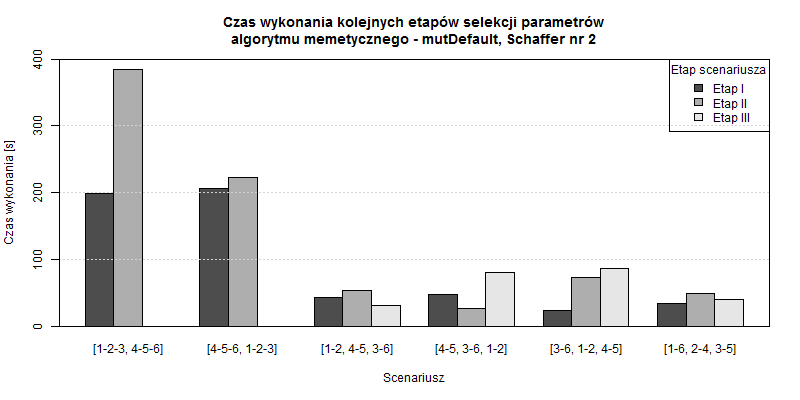
\includegraphics[width=\linewidth]{{img//roz04//parameterSelection//czas_etapow_scenariuszymutDefault_Schaffer1.png}}
  \caption{\emph{mutDefault}}
\end{subfigure}
\begin{subfigure}{\textwidth}
  \centering
  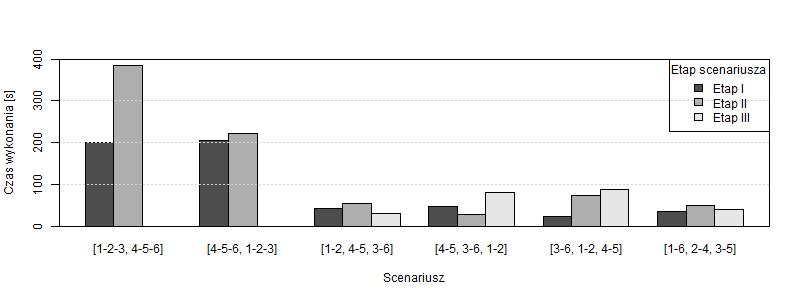
\includegraphics[width=\linewidth]{img//roz04//parameterSelection//czas_etapow_scenariuszymutGauss_Schaffer1.png}
  \caption{\emph{mutGauss}}
\end{subfigure}
\caption{Czas wykonania kolejnych etapów selekcji dla funkcji \emph{Schaffer nr 2}}
\label{fig:parameter_selection_time_in_phases}
\end{figure}

\clearpage

\section{Miary efektywności}
\subsection{Kryterium nr 1 - najlepsze rozwiązanie}

\begin{itemize}
\item we wszystich przypadkach PSO wyszło najgorzej
\item dla Schaffera mutGauss cał zauwazalnie lepsze rezultaty, bo pozniej osiągał zbieżność
\item tam, gdzie nie było problemem znalezienie optymalnego rozwiazania mutGauss osiągał zbieżność wcześniej, a więc szybciej znajdował rozwiązanie
\end{itemize}

\begin{figure}[ht]
\begin{subfigure}{.5\textwidth}
  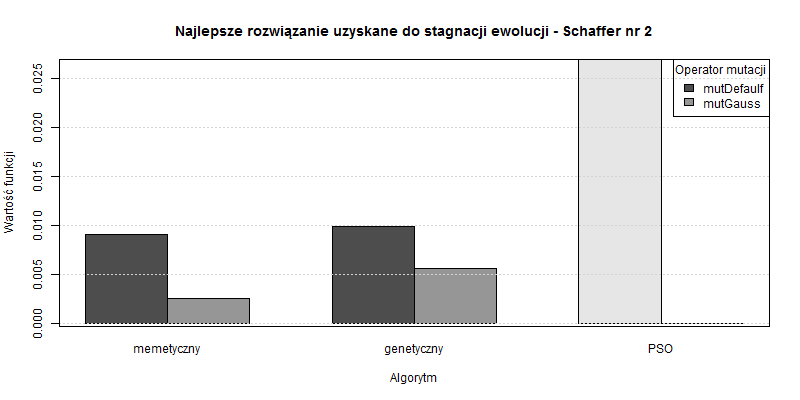
\includegraphics[width=\linewidth]{{img//roz04//kryt1//kryt1_bestFitness_Schaffer.png}}
  \caption{Rozwiązanie stagnacji populacji}
  \label{fig:kryt1_Schaffer_fitness}
\end{subfigure}%
\begin{subfigure}{.5\textwidth}
  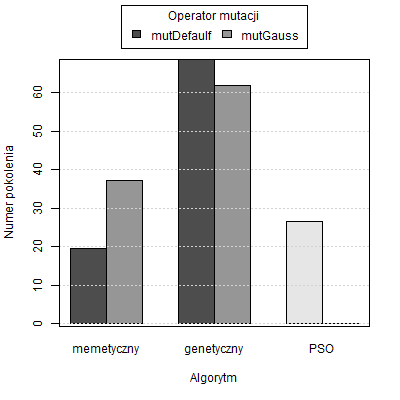
\includegraphics[width=\linewidth]{img//roz04//kryt1//kryt1_nr_generacji_stagnacji_Schaffer.png}
  \caption{Numer pokolenia stagnacji}
  \label{fig:kryt1_Schaffer_stagnation}
\end{subfigure}
\caption{Określenie momentu stagnacji optymalizacji - \emph{Schaffer nr 2}}
\label{fig:kryt1_Schaffer}
\end{figure}

%%%%%%%%%%%%%%%%%%%%%%%%%%%%%%%%%%%%%%%%%%

\begin{figure}[ht]
\begin{subfigure}{.5\textwidth}
  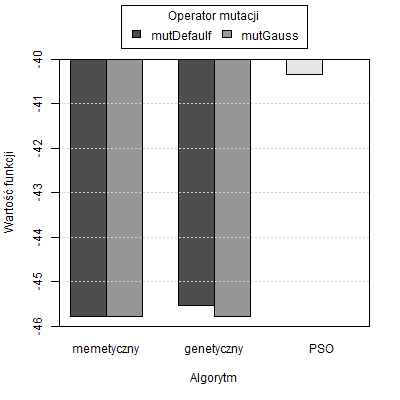
\includegraphics[width=\linewidth]{{img//roz04//kryt1//kryt1_bestFitness_Paviani.png}}
  \caption{Rozwiązanie stagnacji populacji}
  \label{fig:kryt1_Paviani_fitness}
\end{subfigure}%
\begin{subfigure}{.5\textwidth}
  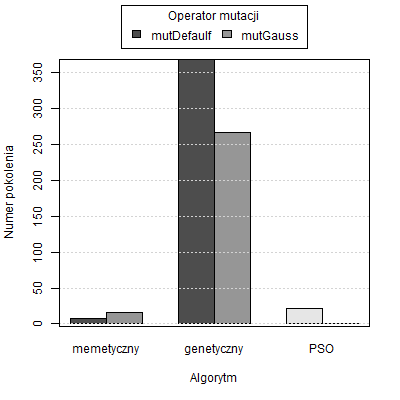
\includegraphics[width=\linewidth]{img//roz04//kryt1//kryt1_nr_generacji_stagnacji_Paviani.png}
  \caption{Numer pokolenia stagnacji}
  \label{fig:kryt1_Paviani_stagnation}
\end{subfigure}
\caption{Określenie momentu stagnacji optymalizacji - \emph{Paviani}}
\label{fig:kryt1_Paviani}
\end{figure}

W Pavianim algorytm genetyczny nie uzyskiwał wartości optymalnej, a inne lokalne optimum o bardzo bliskiej wartości. 

\begin{table}[ht]
\caption{Rozwiązania dla funkcji Paviani}
\label{table:kryt1_Paviani_best_fitness}
\begin{center}
\begin{tabular}{|c|c|c|c|c|c|}
	\hline
	\multirow{2}{*}{Funkcja}& \multicolumn{2}{c|}{Operator mutacji} \\
	\cline{2-6}
	{} & mutDefault & mutGauss \\
	\hline
	\emph{Memetyczny} & -45.77847 & -45.77847\\
	\emph{Genetyczny} & -45.53228 & -45.77498\\
	\emph{PSO} & \multicolumn{2}{c|}{-40.45703}\\
	\hline
	\end{tabular}
\end{center}
\end{table}

           mutDefaulf  mutGauss
memetyczny  -45.77847 -45.77847
genetyczny  -45.53228 -45.77498
PSO         -40.35703   0.00000


%%%%%%%%%%%%%%%%%%%%%%%%%%%%%%%%%%%%%%%%%%

\begin{figure}[ht] 
\begin{subfigure}{.5\textwidth}
  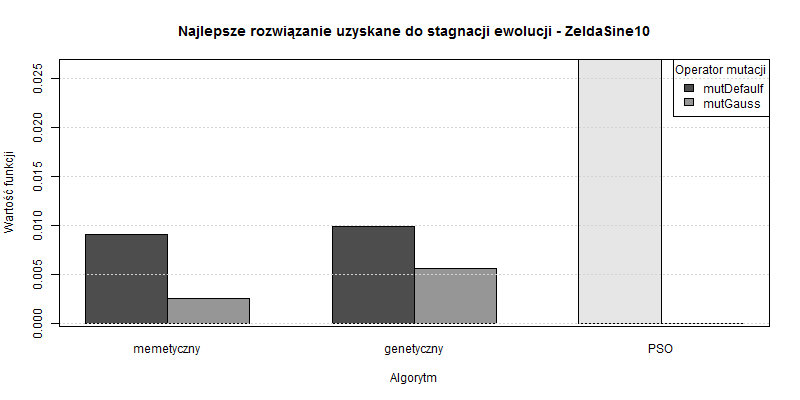
\includegraphics[width=\linewidth]{{img//roz04//kryt1//kryt1_bestFitness_Zeldasine.png}}
  \caption{Rozwiązanie stagnacji populacji}
  \label{fig:kryt1_Zeldasine_fitness}
\end{subfigure}%
\begin{subfigure}{.5\textwidth}
  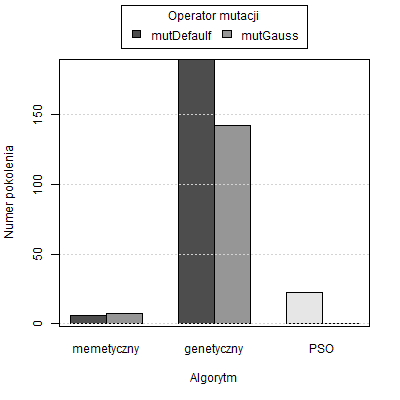
\includegraphics[width=\linewidth]{img//roz04//kryt1//kryt1_nr_generacji_stagnacji_Zeldasine.png}
  \caption{Numer pokolenia stagnacji}
  \label{fig:kryt1_Zeldasine_stagnation}
\end{subfigure} 
\caption{Określenie momentu stagnacji optymalizacji - \emph{ZeldaSine10}}
\label{fig:kryt1_Zeldasine}
\end{figure}




\clearpage

\subsection{Kryterium nr 2 - szybkość osiągania rozwiązania}

\begin{itemize}
\item z uwagi na dużo dłuższe czasy dla PSO i progu 99\% zamieszczono dwa wykresy dla każdej funkcji
\item nieosiągnięcie przez algorytm danego progu w ciągu 30 sekund prezentowane jest jako wartość -0.1
\item nietypowym rezultatem jest nieosiągnięcie przez algorytm memetyczny-mutDefault dla Schaffera progu 99\%
\item najlepsze rezultaty uzyskano algorytmem memetycznym, a w szczególności z wykorzystaniem mutGauss
\item ewidentnie PSO ma problem z optymalizacją Zeldasine, nawet nie uzyskał progu 50\%
\end{itemize}



\begin{table}[ht]
\caption{Wartości kolejnych progów dokładności rozwiązania}
\label{table:kryt2_wartosci_progow}
\begin{center}
\begin{tabular}{|c|c|c|c|c|c|}
	\hline
	\multirow{2}{*}{Funkcja}& \multicolumn{5}{c|}{Próg} \\
	\cline{2-6}
	{} & 50\% & 75\% & 90\% & 95\% & 99\% \\
	\hline
	\emph{Schaffer nr 2} & 0.25227 & 0.12614 & 0.05045 & 0.02523 & 0.00504\\
	\emph{Paviani} & -22.42884 & -34.10365 & -41.10854 & -43.44351 & -45.31148\\
	\emph{ZeldaSine10} & -1.92663 & -2.71331 & -3.18532 & 3.34266 & 3.46853\\
	\hline
	\end{tabular}
\end{center}
\end{table}


%%%%%%%%%%%%%%%%%%%%%%%%%%%%%%%%%%%%%%%%%
\begin{figure}[ht] 
\centering
\begin{subfigure}{\textwidth}
  \centering
  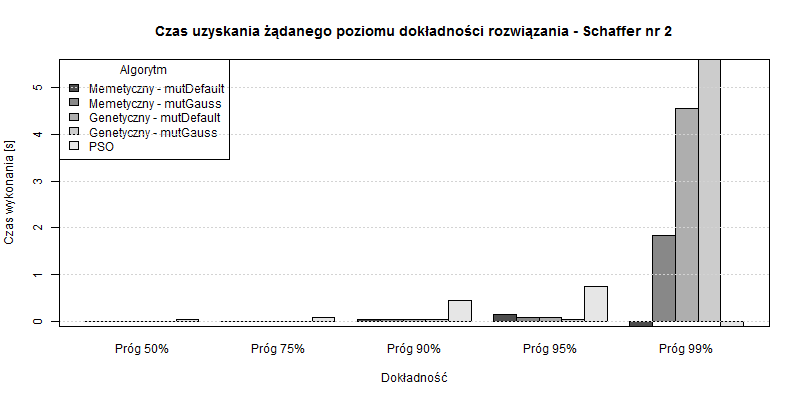
\includegraphics[width=\linewidth]{{img//roz04//kryt2//kryt2_czas_uzyskania_poziomu_dokladnosci_Schaffer.png}}
  \caption{Wszystkie algorytmy i progi dokładności}
\end{subfigure} 
\begin{subfigure}{\textwidth}
  \centering
  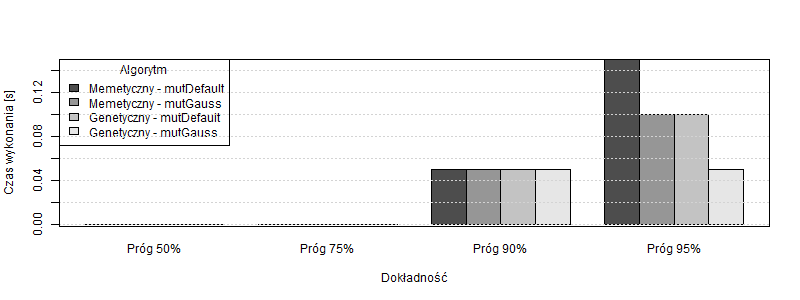
\includegraphics[width=\linewidth]{img//roz04//kryt2//kryt2_czas_uzyskania_poziomu_dokladnosci_bez_PSO_Schaffer.png}
  \caption{Wszystkie algorytmy i progi dokładności z wyłączeniem PSO i progu 99\%}
\end{subfigure} 
\caption{Czas osiągnięcia rozwiązania o zadanej dokładności - \emph{Schaffer nr 2}}
\label{fig:kryt2_Schaffer}
\end{figure}
%%%%%%%%%%%%%%%%%%%%%%%%%%%%%%%%%%%%%%%%%%%%
%
%%%%%%%%%%%%%%%%%%%%%%%%%%%%%%%%%%%%%%%%%%
\begin{figure}[ht] 
\centering
\begin{subfigure}{\textwidth}
  \centering
  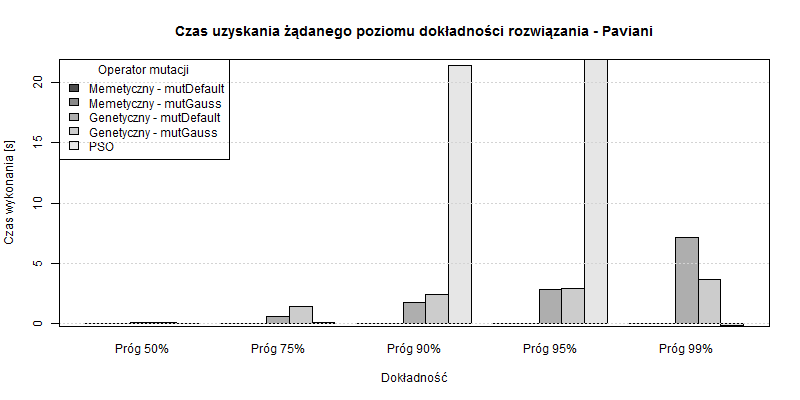
\includegraphics[width=\linewidth]{{img//roz04//kryt2//kryt2_czas_uzyskania_poziomu_dokladnosci_Paviani.png}}
  \caption{Wszystkie algorytmy i progi dokładności}
\end{subfigure}
\begin{subfigure}{\textwidth}
  \centering
  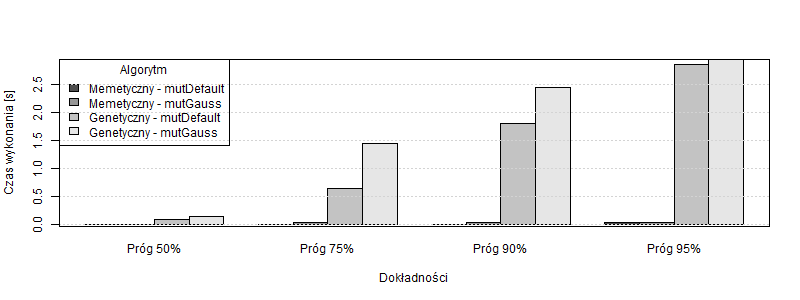
\includegraphics[width=\linewidth]{img//roz04//kryt2//kryt2_czas_uzyskania_poziomu_dokladnosci_bez_PSO_Paviani.png}
  \caption{Wszystkie algorytmy i progi dokładności z wyłączeniem PSO i progu 99\%}
\end{subfigure}
\caption{Czas osiągnięcia rozwiązania o zadanej dokładności - \emph{Paviani}}
\label{fig:kryt2_Paviani}
\end{figure}
%%%%%%%%%%%%%%%%%%%%%%%%%%%%%%%%%%%%%%%%%%%
%
%%%%%%%%%%%%%%%%%%%%%%%%%%%%%%%%%%%%%%%%%%
\begin{figure}[ht] 
\centering
\begin{subfigure}{\textwidth}
  \centering
  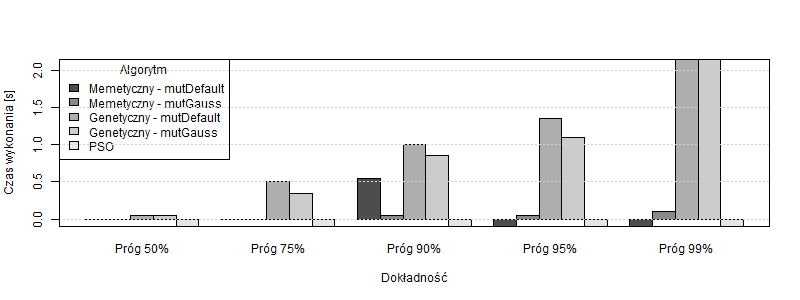
\includegraphics[width=\linewidth]{{img//roz04//kryt2//kryt2_czas_uzyskania_poziomu_dokladnosci_Zeldasine.png}}
  \caption{Wszystkie algorytmy i progi dokładności}
\end{subfigure} 
\begin{subfigure}{\textwidth}
  \centering
  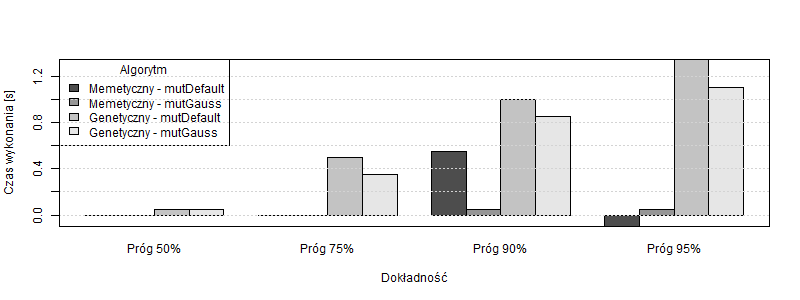
\includegraphics[width=\linewidth]{img//roz04//kryt2//kryt2_czas_uzyskania_poziomu_dokladnosci_bez_PSO_Zeldasine.png}
  \caption{Wszystkie algorytmy i progi dokładności z wyłączeniem PSO i progu 99\%}
\end{subfigure} 
\caption{Czas osiągnięcia rozwiązania o zadanej dokładności - \emph{ZeldaSine10}}
\label{fig:kryt2_Zeldasine}
\end{figure}
%%%%%%%%%%%%%%%%%%%%%%%%%%%%%%%%%%%%%%%%%%



\clearpage
\subsection{Kryterium nr 3 - powtarzalność skutecznej optymalizacji}

\begin{itemize}
\item operator mutDefault w porównaniu do mutGauss dla Schaffera wypadł bardzo słabo, dla poziomu 0.01 nawet PSO uzyskało wyższą powtarzalność uzyskania rozwiązania danej dokładności niz algorytmu z mutDefault
\item w Pavianim 
\end{itemize}


%%%%%%%%%%%%%%%%%%%%%%%%%%%%%%%%%%%%%%%%%%%%%%%
\begin{figure}[ht] 
\centering
  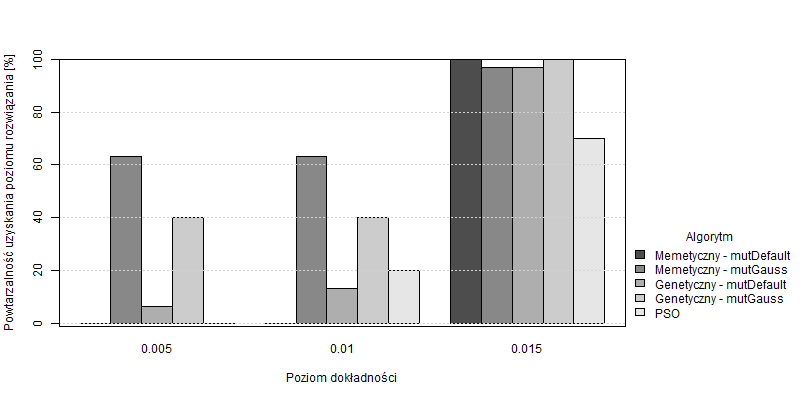
\includegraphics[width=\linewidth]{{img//roz04//kryt3//kryt3_czas_uzyskania_poziomu_dokladnosci_Schaffer.png}}
\caption{Powtarzalność uzyskania rozwiązania o danej dokładności - \emph{Schaffer~nr~2}}
\label{fig:kryt3_Schaffer}
\end{figure}
%%%%%%%%%%%%%%%%%%%%%%%%%%%%%%%%%%%%%%%%%%%%%

%%%%%%%%%%%%%%%%%%%%%%%%%%%%%%%%%%%%%%%%%%%%%%%
\begin{figure}[ht] 
\centering
  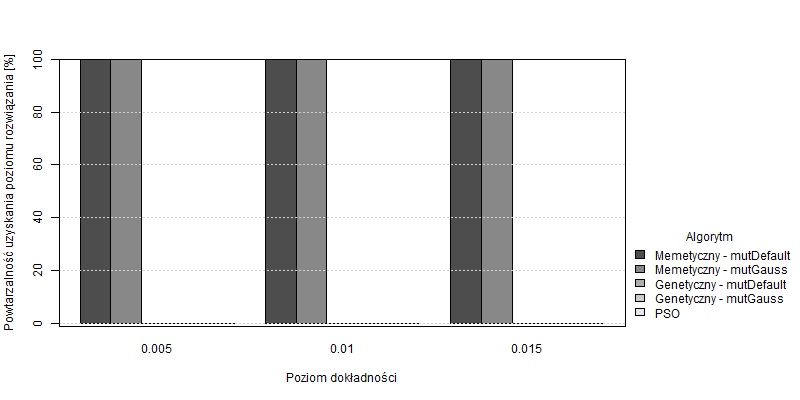
\includegraphics[width=\linewidth]{{img//roz04//kryt3//kryt3_czas_uzyskania_poziomu_dokladnosci_Paviani.png}}
\caption{Powtarzalność uzyskania rozwiązania o danej dokładności - \emph{Paviani}}
\label{fig:kryt3_Paviani}
\end{figure}
%%%%%%%%%%%%%%%%%%%%%%%%%%%%%%%%%%%%%%%%%%%%%


%%%%%%%%%%%%%%%%%%%%%%%%%%%%%%%%%%%%%%%%%%%%%%%
\begin{figure}[ht] 
\centering
  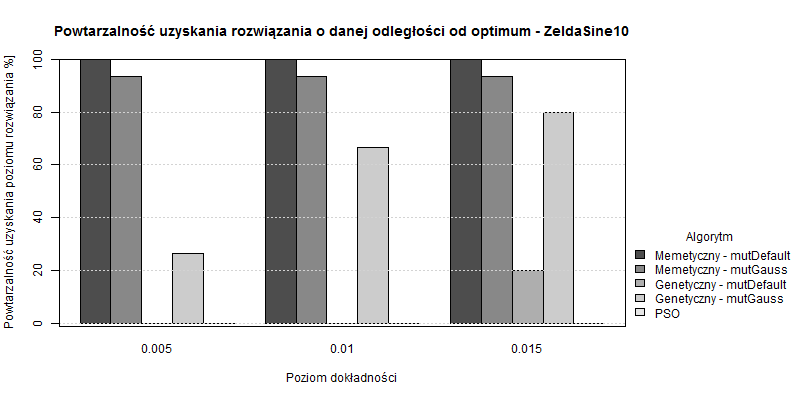
\includegraphics[width=\linewidth]{{img//roz04//kryt3//kryt3_czas_uzyskania_poziomu_dokladnosci_Zeldasine.png}}
\caption{Powtarzalność uzyskania rozwiązania o danej dokładności - \emph{ZeldaSine10}}
\label{fig:kryt3_Zeldasine}
\end{figure}
%%%%%%%%%%%%%%%%%%%%%%%%%%%%%%%%%%%%%%%%%%%%%

\clearpage
\subsection{Kryterium nr 4 - ogólna charakterystyka populacji}


%%%%%%%%%%%%%%%%%%%%%%%%%%%%%%%%%%%%%%%%%%%%%%%
\begin{figure}[ht] 
\centering
  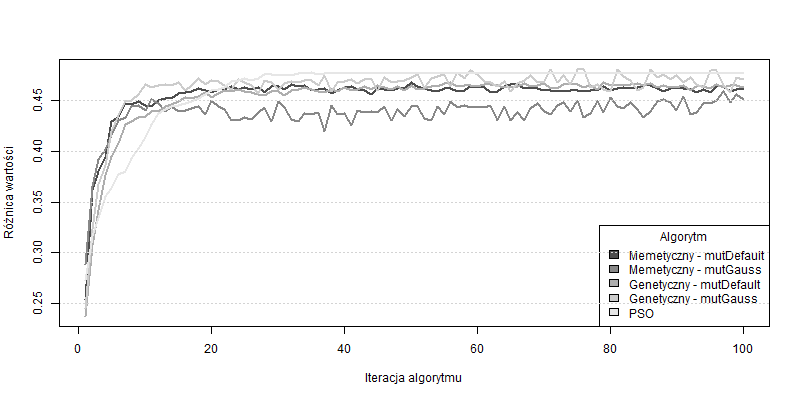
\includegraphics[width=\linewidth]{{img//roz04//kryt4//kryt4_czas_uzyskania_poziomu_dokladnosci_Schaffer.png}}
\caption{Różnica pomiędzy średnim i najlepszym rozwiązaniem populacji w kolejnych iteracjach algorytmu - \emph{Schaffer~nr~2}}
\label{fig:kryt4_Schaffer}
\end{figure}
%%%%%%%%%%%%%%%%%%%%%%%%%%%%%%%%%%%%%%%%%%%%%

%%%%%%%%%%%%%%%%%%%%%%%%%%%%%%%%%%%%%%%%%%%%%%%
\begin{figure}[ht] 
\centering
  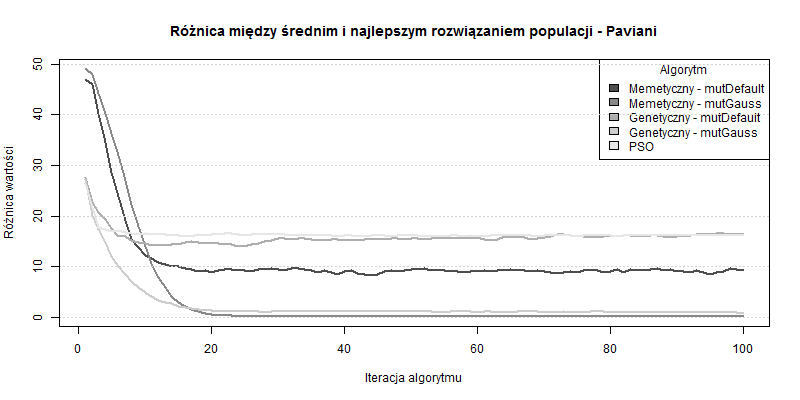
\includegraphics[width=\linewidth]{{img//roz04//kryt4//kryt4_czas_uzyskania_poziomu_dokladnosci_Paviani.png}}
\caption{Różnica pomiędzy średnim i najlepszym rozwiązaniem populacji w kolejnych iteracjach algorytmu  - \emph{Paviani}}
\label{fig:kryt4_Paviani}
\end{figure}
%%%%%%%%%%%%%%%%%%%%%%%%%%%%%%%%%%%%%%%%%%%%%


%%%%%%%%%%%%%%%%%%%%%%%%%%%%%%%%%%%%%%%%%%%%%%%
\begin{figure}[ht] 
\centering
  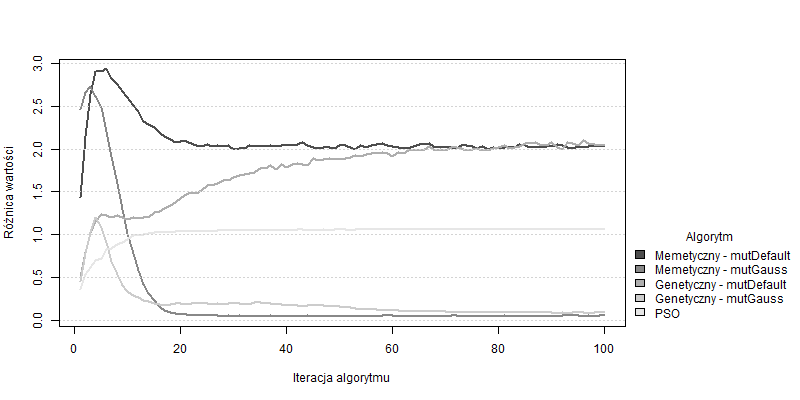
\includegraphics[width=\linewidth]{{img//roz04//kryt4//kryt4_czas_uzyskania_poziomu_dokladnosci_Zeldasine.png}}
\caption{Różnica pomiędzy średnim i najlepszym rozwiązaniem populacji w kolejnych iteracjach algorytmu  - \emph{ZeldaSine10}}
\label{fig:kryt4_Zeldasine}
\end{figure}
%%%%%%%%%%%%%%%%%%%%%%%%%%%%%%%%%%%%%%%%%%%%%